\chapter{Lecture 22}\label{chap22}

\setcounter{section}{36}
\section{Constant Field Extensions}\label{chap22:sec37}%Sec 37

We\pageoriginale require some preliminary lemmas.
\setcounter{Lemma}{0}
\begin{Lemma}\label{chap22:sec37:lem1}%Lem 1
  Let $A, B$ and $C$ be subfields of a given field, $B \supset A$ and
  $C$ algebraic of finite degree $n$ over  $A$. Then the composite
  extension $BC$ is algebraic over $B$ of degree at most $n$. Moreover
  if $y_1, \ldots y_n$ is a basis of $C$ over $A, BC$ is spanned by
  the same set of elements $y_1 , \ldots y_n$ over $B$. The degree of
  $BC$ over $B$ is equal to $n$ if and only if $B$ and $C$ are
  linearly disjoint over $A$. 
\end{Lemma}

\begin{proof}
  Since $y_1, \ldots  y_n$ span $C$ over $A$, we have in particular $C
  = A(y_1$, $\ldots$, $y_n)$ and since $B \supset A, ~ BC = B(y_1, \ldots
  y_n)$. Hence any element of $BC$ can be written as a polynomial in
  $y_1 , \ldots y_n$ with coefficients in $B$ (since $y_1 , \ldots
  y_n$ are algebraic over $A$),  and since any monomial in $y_1 ,
  \ldots , y_n$ can be written as a linear combination of $y_1 ,
  \ldots , y_n$ with coefficients in $A$, we deduce that $BC$ is the
  vector space spanned by $y_1, \ldots .. y_n$ over $B$. Hence $[ BC :
    B ] \le n$. 
\end{proof}

If $[BC : B] = n, y_1 , \ldots y_n$ should also be linearly
independent over $B$, and since $(y_1, \ldots y_n)$ is an arbitrary
set of $n$ elements of $C$ linearly independent over $A, B$ and $C$
are linearly disjoint over $A$. The converse is also evident. 

\begin{Lemma}\label{chap22:sec37:lem2}%Lem 2
  \begin{enumerate}[(a)]
  \item Let $B$ be any purely transcendental extension of $A$ and $C $
    any\pageoriginale field containing $A$ and algebraically disjoint
    with $B$ over 
    $A$. Then $C$ and $B$ are linearly disjoint over $A$. 
  \item Let $A$ be algebraically closed in $B$ and $C = A (\alpha)$ a
    simple algebraic extension of $A$. Then $B$ and $C$ are linearly
    disjoint over $A$. 
  \end{enumerate}
\end{Lemma}

\begin{proof}
  \begin{enumerate} [(a)]
  \item Let $B = A(u_\lambda)_{ \lambda \in A}$ where
    $u_\lambda$ is a set of algebraically independent elements over
    $A$. If $B$ and $C$ are not linearly disjoint, there is a set of
    elements $c_1, \ldots c_n \in C$ which are linearly independent
    over $A$ and polynomials $f_i (u_1 , \ldots u_m ), u_i, \in
    \{u_i\}_{\lambda \in A}$ not all of which vanish identically
    such that 
    $$
    c_1 f_1 (u_1 , \cdots u_m ) + \cdots + c_n f_n (u_1 , \ldots u_m)
    = 0, f_i \in A[u_1 , \ldots , u_m] 
    $$
    Since $u_1 , \ldots u_m$ are algebraically independent over $A$,
    they are algebraically independent over $C$ also. We may therefore
    equate to zero separately the coefficients of each of the monomial
    expressions in $u_1 , \ldots u_m$ occurring in the left hand side
    of the above equation. At least one of these provides a
    non-trivial linear combination of the $c_i$ with coefficients in
    $A$ which vanishes. This is a contradiction. 
  \item Since $A$ is algebraically closed in $B$, the irreducible
    monic polynomial of $\alpha$ over $B$ is actually a polynomial
    over $A$, as we have proved earlier. Hence $[ B(\alpha) : B ] = [A
      (\alpha) : A]$, and our result follows from Lemma $1$. 
  \end{enumerate}
\end{proof}

\begin{Lemma}\label{chap22:sec37:lem3}%Lem 3
  Let $A, B, C, D$ be subfields of a given field such that $B \supset
  A, D \supset C \supset A$.\pageoriginale Then $B$ and $D$ are linearly disjoint
  over $A$ if and only if $(i) B$ and $C$ are linearly disjoint and
  (ii) $D$ and the composite extension $BC$ are linearly disjoint over
  $C$. 
\end{Lemma}

\begin{proof}
  Suppose first that $B$ and $D$ are linearly disjoint. Then $(i)$ is
  evidently fulfilled. To prove $(ii)$, suppose $d_i (i = 1, \ldots
  n)$ is a set of elements of $D$ linearly independent over $C$. If
  they are linearly dependent over $BC$, there exists a relation of
  the form 
  $$
  \sum_i d_i \sum_j c_{ij} b_j = 0 ~ , c_{ij} \in C, b_j \in B,
  $$
  with $b_j$ linearly independent over $C$ and not all $c_{ij} $ being
  zero. On interchanging the orders of summation, we get 
  $$
  \sum_j b_j \sum_j d_i c_{ij} = 0,
  $$
  and we deduce from our hypothesis that
  $$
  \sum_i c_{ij } d_i = 0 \quad \text{for all} ~~j.
  $$
\end{proof}

But since $d_i$ are linearly independent over $C$, we have $c_{ij} =
0$ for all $i $ and $j$. This is a contradiction. 

Suppose conversely that $(i)$ and $(ii)$ are fulfilled. Then any set
of elements of $B$ linearly independent over $A$ are, by $(i)$,
linearly independent over $C$, and (since they are also elements of
$BC)$ by $(ii)$, linearly independent over $D$. Our lemma is proved. 

We can now prove the following

\begin{theorem*}
  Let $L = Kl_0$ be a constant field extension of $K$ with the\pageoriginale field
  of constants $l \supset l_0$. Then the following conditions are
  equivalent 
  \begin{enumerate} [(A)]
  \item $K$ and $l$ are linearly disjoint over $k$.
  \item  For every finitely generated subfield $l'_0 $ of $l_0$ over
    $k$, and $L^1 = Kl_0^1$, the constant field of $L^1$ coincides
    with $1^1_0$. 
  \end{enumerate}
\end{theorem*}

If these are fulfilled, $(B)$ holds for any (not necessarily finitely
generated) subfield $l^1_0$ of $l_0$, in particular for $l_0$ itself,
i,e., $l = l_0$. 

\begin{proof}
  We shall first show that $(A)$ implies $(B)$ for any subfield
  $l_0^1$ of $l_0$. Let $l^1$ be the constant field of $L^1 =
  Kl_0^1$. It follows from $(A)$ that $l^1$ and  $K$ are linearly
  disjoint over $k$. 

  Let $X$ be any transcendental element of $K$ over $k$. Then by Lemma
  \ref{chap22:sec37:lem3}, $K$ and $1^1$ are linearly disjoint over $k$ if and only if
  (i) $k(X)$ and $l^1$ are linearly disjoint over $k$ and (ii) $K$
  and $l^1 k(X) = l^1 (X)$ are linearly disjoint over $k(X)$. 

  By lemma \ref{chap22:sec37:lem2}, since $k(X)$ are $1^1$ are
  algebraically disjoint   (i) is always satisfied. By
  lemma \ref{chap22:sec37:lem1}, since 
  $1^1_0 (X) \subset   1^1 (X)$ and $L^1 = K1^1_0 (X)$, we have the inequalities 
  \begin{figure}[H]
    \centerline{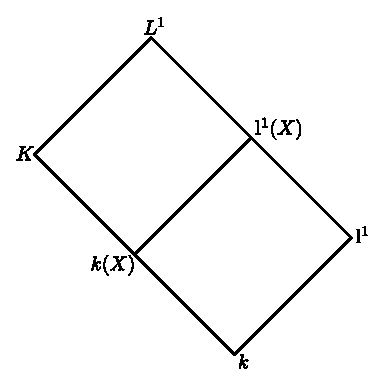
\includegraphics{vol18-figures/fig18.1.eps}}
  \end{figure}
  $$
  \big [ L^1 : l^1 (X) \big ] \le \big [L^1 : l^1_o (X) \big ] \le
  \big [K : k(X) \big]. 
  $$
\end{proof}

Again by lemma \ref{chap22:sec37:lem1}, since $L^1 = Kl^1 (X)$, the equality
$$
\big [ L^1 : l^1 (X) \big ] = \big [ K : k(X) \big]
$$
follows from the linear disjointness of $K$ and $l^1(X)$ over $k(X)$.

From\pageoriginale these we deduce that if $(A)$ holds, $l^1 (X) = l^1_0 (X)$, and
since $X$ is transcendental over $l^1 , l^1 = l^1_0$. 

Conversely suppose $(B)$ holds for every finitely generated subfield
$l^1_0$ of $l_0$. To prove that $1$ and $K$ are linearly disjoint, it
is enough to prove that any finitely generated subfield of $1$ over
$k$ is linearly disjoint with $K$ over $k$. But clearly a  finitely
generated subfield of $l$ is contained in the constant field $l^1 =
l^1_0$ of $L^1 = Kl^1_0$, where $l^1_0$ is a suitable finitely
generated extension of $k$. It is therefore enough to prove that any
finitely generated subfield $l^1_0$ of $l_0$ over $k$ is linearly
disjoint with $K$ over $k$. 

Let $l^1_0 = k(\alpha_1 , \ldots \alpha_m)$. Put $k_i = k(\alpha_1 ,
\ldots \alpha_i)$, and $l_i = K k_i$. To show that $l^1_0$ and $K$ are
linearly disjoint over $k$, it is enough to show that $k_1$ and $K$
are linearly disjoint over $k, k_2$ and $L_1 = K K_1$ are linearly
disjoint over $k_1$, etc., and finally $l^1_0 = k_m$ and $L_{m - 1} =
K Kk_{m - 1}$ are linearly disjoint over $k_{m-1}$ (Lemma \ref{chap22:sec37:lem3}). But by
$(B)$ each $k_i$ is algebraically closed in $L_i$ and since $k_{i + 1}
$ is a simple extension of $k_i$, our result follows from Lemma $2$. 
  \begin{figure}[H]
    \centerline{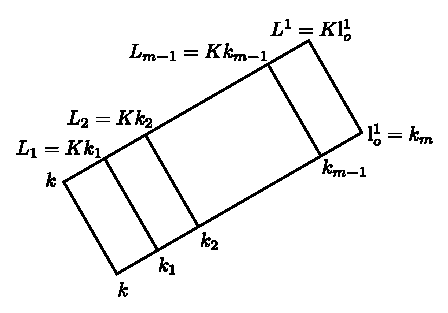
\includegraphics{vol18-figures/fig18.2.eps}}
  \end{figure}

\begin{coro*}%Corlry
  If either $K$ or $l_0$ is separably generated over $k$, then $l=l_0$.
\end{coro*}

\begin{proof}
  By the above theorem, we may assume that $l_0$ is finitely generated
  over $k$. Morover, since we have already seen that $l= l_0$ for\pageoriginale a
  purely transcendental extension $l_0$ of $k$ (see Lecture \ref{chap21}), we
  may assume that $l_0$ is finitely algebraic over $k$. 
\end{proof}

Suppose now that $l_0$ is separably algebraic over $k$. Then $L =
Kl_0$ is separably algebraic over $K$. But if $\alpha \in l$, the
irreducible monic polynomial of $\alpha$ over $K$ lies in $k$ and is
therefore separable over $k$. Hence $l$ is separable over $l_0$, and
is also purely inseparable $l = l_0$. 

Suppose next that $K$ is separably generated over $k$. Let $X \in K$
be transcendental over $k$ and such that $K/k(X)$ is separable. Then
$L = Kl_0 (X)$ is separable over $l_0(X)$. Hence any element of $l$ is
separably algebraic over $l_0(X)$, and since $l_0$ is algebraically
closed in $l_0(X), l$ is separable over $l_0$. The result follows as
before. 

Our next theorem runs as follows.

\begin{theorem*}
  Let $L = l_0 K$ be a constant field extension and $\lambda_{L/K}$
  the rational number satisfying 
  $$
  \lambda_{L/K} d_L (\mathscr{U}) = d_K (\mathscr{U})
  $$
  for any divisor $\mathscr{U}$ of $K$. Then $\lambda_{L/K}$ is a
  power of the characteristic with non-negative exponent
  $(\lambda_{L/K} = 1$ if the characteristic is zero). It is equal to
  one if and only if $K$ and $l$ are linearly disjoint over $k$. 
\end{theorem*}

\begin{proof}
  Let $X$ be a transcendental element of $K$. Choose $\mathscr{U}$ to
  be the numerator of $(X)$. Then, we see that 
  $$
  d_K(\mathscr{U}) = [K : k(X)] ~ \text{and} ~ d_L (\mathscr{U}) = [L : l(X)]
  $$
  
  Hence,\pageoriginale\
  $$
  \lambda_{L/K} = 1 \Leftrightarrow d_L(\mathscr{U}) =
  d_K(\mathscr{U}) \Leftrightarrow [L : l(X)] = [K : k(X)]. 
  $$

  But as we have already seen (see proof of the first theorem of this
  lecture) $[L : l(X)] = [K : k(X)]$ if and only if $K$ and $l$ are
  linearly disjoint over $k$. 
\end{proof}

In particular, if the characteristic is zero, $K$ is separably
generated over $k$, and by the corollary of the first theorem, the
condition (B) of our first theorem is satisfied. Hence (A) holds,
i.e., $K$ and $l$ are linearly disjoint over $k$. Hence $\lambda_{L
  /K} = 1$.  

If the characteristic $p > 0$, let $K_0$ be the largest separable
extension of $k (X)$ contained in $K$, and $L_0 = K_0 l_0$. Then as
above, $K_0$ and $l_0$ are linearly disjoint over $k$. Hence we obtain  
$$
\big[ K_0 : k (X) \big] = \big[L_0 : l_0 (X)\big]
$$

Also, $K/K_0$ is a purely inseparable extension of degree $p^s, s \ge
0$ and therefore so is $L =Kl_0$ inseparable of degree $p^s$, where
$s_0 \le s$ (lemma \ref{chap22:sec37:lem1}). Therefore we have  
\begin{align*}
  \lambda_{L/K} & = \frac{\big[ K: k (X)\big]} {\big[ L : l(X)\big]}
  = \frac{\big[ K : k (X)\big] \big[l(X) : l_0 (X)\big]} {\big[ L :
      l_0 (X)\big]}\\ 
  & = \frac{\big[ K : K_0\big] \big[ K_0 : k (X)\big]} {\big[ L
      :L_0\big] \big[ L_0 :l_0 (X)\big]} \big[ l : l_0\big] =
  p^{s-s_0} \big[ l: l_o\big] 
\end{align*}

Thus, we see that $\lambda_{L/K}$ is a power of $p$ divisible by
$\big[ l:l_0\big]$. Our\pageoriginale theorem is proved. 

In particular, we see that if $K$ or $l_0$ is separably
generated over $k, K$ and $l$ are linearly disjoint over $k$ and
therefore $\lambda_{L/K} = 1$.  
 
The last theorem of this section relates to the residue class field of
a prime divisor in a constant filed extension. 

\begin{theorem*}
  Let $L = Kl$, where $I$ is separably generated over $k$. If
  $\mathscr{K}$ is a prime divisor of $L$ lying over the prime divisor
  $\mathscr{Y}$ of $K$, $L_\mathscr{R}$ is the composite of the two
  subfields $K_\mathscr{Y}$ and $l$. 
\end{theorem*}

\begin{proof}
  It is clearly sufficient to prove the theorem when (1) $l$ is purely
  transcendental over $k$ and (2) when $l$ is separably algebraic
  over $k$.  
\end{proof}

\setcounter{Case}{0}
\begin{Case}%Case 1
  Since $K_\mathscr{Y}$ is algebraic over $K, l$ and $K_\mathscr{Y}$
  are linearly disjoint over $k$. Let us agree to denote the image in
  $L_\mathscr{K}$ of any element $Y$ in the valuation ring
  $\mathscr{O}_\mathscr{K}$ by $\bar{Y}$. Any $Y \in
  \mathscr{O}_\mathscr{K}$ can be written in the form  
  $$
  \frac{\sum\limits_{i=1}^n k_i l_i}{\sum\limits_{j=1}^m k^1_j l^1_j}
  ,\quad  k_i, k^1_j \in K, l_i, l^1_j \in 1, 
  $$ 
  and the two sets of elements $(l_i)$ and $(l^1_j)$ being linearly
  independent over $k$. Find elements $a, b ~\text{ of }~ K$ such that
  $v_\mathscr{Y} (a) = \min\limits_{i=1}^n v_\mathscr{Y} (k_i) \text{
    and } v_\mathscr{Y} (b) = -\min\limits_{j=1}^m v_\mathscr{Y}
  (k^1_j)$. Then clearly for at least one $j\, v_\mathscr{Y}  (k_j^1 b)
  = 0, k^1_j \neq 0$. The image $L_{\mathfrak{R}}$ of the element
  $\dfrac{aY}{b}$\pageoriginale is then   
  $$
  \frac{\sum \overline{(k_i a)} l_i}{\sum \overline{(k^1_j b)} l^1_j}
  $$
  Since the $l_i$ are linearly independent over $k$, they are also
  linearly independent $K_\mathscr{Y}$ and therefore the numerator
  does not vanish. Similarly the denominator does not vanish, and
  therefore the image of $\dfrac{aY}{b}$ in $L_{\mathscr{K}}$ is a
  non-zero element of $K_\mathscr{Y} l$. Since $Y \in
  \mathscr{O}_\mathscr{K}$, it follows that $\dfrac{b}{a} \in
  \mathscr{O}_\mathscr{Y}$ and hence $\bar{Y} = \left(\dfrac{\bar b}{\bar{
  a}}\right) \left(\dfrac{\bar{aY}}{\bar b}\right) \in K_\mathscr{Y} l$.     
\end{Case}

Since $K_\mathscr{Y}$ and $l$ are linearly disjoint, the structure of
$L_\mathscr{K}$ is uniquely determined; in fact $L_\mathscr{K}$ is
purely transcendental over $K$, and a transcendence basis of $l$ over
$k$ is also a transcendence basis of $L_\mathscr{K}$ over
$K_\mathscr{Y}$. Since the map $Y\to \bar{Y}$ is also uniquely fixed,
we see that there is exactly one prime divisor $\mathscr{K}$ of $L$
lying over the prime divisor $\mathscr{Y}$ of $K$.  

\begin{Case}%Case 2
  In this case we may not only assume that $l$ is separably algebraic
  over $k$, but also that it is finite. In fact, any element $\alpha$
  of $L_\mathscr{K}$ is clearly the image by the place of
  $\mathscr{K}$ of an element of $Kl^1$, where $l^1$ is a finite
  extension of $k$. If we have proved the theorem for finite separable
  extensions, it would follow that $\alpha \in l^1
  K_\mathscr{Y} \subset lK_\mathscr{Y}$ and we would be through.   
\end{Case}

Suppose $l$ is separably algebraic and of finite degree over $k$. Then
it is simple and we have $l = k (\alpha)$, where $\alpha$ is separably
algebraic over $k$ of degree $n$, say. Let $\mathscr{K} =
\mathscr{K}_1, \mathscr{K}_2 ,\ldots, \mathscr{K}_n$ be all\pageoriginale the prime
divisors of $L$ lying over $\mathscr{Y}$. Let $L^1$ be the smallest
normal extension of $K$ containing $L$, and $\mathscr{K}^1$ a prime
divisor of $L^1$ lying over $\mathscr{K}$. Let $\sigma_i (i=1
,\ldots,m)$ be all the automorphisms of $L^1$ over $K$. Then since
$\sigma_i \mathscr{K}^1$ again lies over the prime divisor of $K$, its
restriction to $L$ is one of the $\mathscr{K}_j$.  

Let $\bar{Z} \in L_\mathscr{K}$. Find an element  $C \in L$ such that   
$$
\displaylines{\hfill
  v_\mathscr{K} (C -Z) >0,\hfill \cr
  \text{and} \hfill  v_\mathscr{K}{_{j}} (C) \ge 0,  (j =2 ,\ldots
  h)\hfill }
$$

By the first condition , $\bar{C} = \bar{Z} \in L_\mathscr{K}$.

Since $C \in K(\alpha)$, it can be written uniquely in the form
$$
C= a_o + a_1 \alpha +\cdots \cdots+ a_{n-1} \alpha^{n-1} , a_i \in K
$$
(the degree of $\alpha$ over $K$ being the same as over $k$, according
to a previous statement). 

Taking conjugates in the above equation over $K$, we obtain a set of
$n$ equations 
$$
C^{(i)} = a_0 + a_1 \alpha^{(i)} +\cdots \cdots+ a_{n-1} \alpha
^{(i)^{n-1}} 
$$

Since $\alpha$ is separable of degree $n$ over $K$, the determinant
$|\alpha^{(i) j}| (i =1 ,\ldots, n; j=o ,\ldots, n-1)$  has a non-zero
value, and  we may solve the above equations for $a_k$ to obtain 
$$
a_k=\frac{
  \begin{vmatrix} 
    1 \alpha^{(1)} & \cdots  & \alpha^{(1)^{k-2}}C_1 & \cdots &
    \alpha^{(1)^{n-1}} \\  
    1 \alpha^{(n)} & \cdots  & \alpha^{(n)^{k-2}}C^n & \cdots &
    \alpha^{(n)^{n-1}}  
  \end{vmatrix}} 
  {\begin{vmatrix} 
      1 \alpha^{(1)} &  \cdots \cdots \cdots \cdots \cdots \cdots
      \cdots  & \alpha^{(1)^{n-1}}\\ 
      1 \alpha^{(n)} & \cdots \cdots \cdots \cdots \cdots  \cdots
      \cdots & \alpha^{(n)^{n-1}}  
  \end{vmatrix}}
$$\pageoriginale\

The denominator is a constant of the filed $L^1$. The numerator is a
linear combination of the $C^{(i)}$ with constant coefficients.  But we
have 
$$
v_{\mathscr{K}^1} (C^{(i)}) = v_{\sigma_\nu^{-1}
  \mathscr{K}'} (C) = e_{L^1/L} {(\sigma_\nu^{-1} \mathscr{K}^1)}
  v_{\mathscr{K}j} (C) \ge 0 
$$
where $\sigma_\nu$ is an automorphism of $L^1/K$ taking $C$ to
$C^{(i)}$ and $\mathscr{K}_j$ is the prime divisor of $L$ lying below
$\sigma_nu ^{-1} \mathscr{K}^1$.  

We may therefore conclude that
$$
v_{\mathscr{K}^1} (a_k) \ge 0, v_{\mathscr{K}} (a_k) \ge 0
$$

This means that the $a_k$ are in $\mathscr{O}_\mathscr{K}$ and therefore
$$
\bar{Z} = \bar{C} = \bar{a_o} + \bar{a_1} \alpha +\cdots \cdots+
\overline{a_{n-1}} \alpha^{n-1} \in lK_\mathscr{Y}. 
$$

Our theorem is proved.

From the proof of the theorem when $l_0$  is purely transcendental,
the following fact emerges. If $\mathscr{K}$ is a prime divisor of $L
= Kl_0, l_0$ being purely transcendental, and $\mathscr{K}$ lies over
a prime divisor $\mathscr{Y}$ of $K$, we have  
$$
v_\mathscr{K} \left(\sum\limits_1^n l_i a_i\right) = \min^n_{i=1}
(v_\mathscr{Y} (a_i)) 
$$
if\pageoriginale $l_i \in l_0$ and $a_i \in K$. This follows in fact
from the equation 
$$
\overline{\sum_{i=1}^{n} l_i a_i}=\sum_{i=1}^{n}l_i \bar{a}_i, \text{ if } a_i
\in \mathscr{O}_\mathscr{Y}. 
$$
